\chapter{Pygame Invaders: Η Αρχή!}
\label{chap:pygame-invaders-start}
\section{Εισαγωγή}
Αν είχατε ξεκινήσει να προγραμματίζετε στα 80s, είναι σίγουρο ότι τα πρώτα σας προγράμματα θα ήταν παρόμοια με αυτά που έχουμε γράψει ως τώρα. Πολλά μάλιστα θα τα είχατε αντιγράψει από το εγχειρίδιο προγραμματισμού του υπολογιστή σας και σίγουρα θα είχατε σπαταλήσει αρκετές ώρες για να κατανοήσετε πως λειτουργούν και να πειραματιστείτε σε παραλλαγές τους. Αν μάλιστα μας επιτρέπετε να μαντέψουμε, μετά τα πρώτα σας προγράμματα των 5-10 γραμμών, θα είχατε γράψει ένα πρόγραμμα ``Guess the Number'' ένα ``Bouncing Ball'' και ένα παιχνίδι ``Graphics Match''.

Δεν ξέρω αν η πορεία αυτή σας θυμίζει κάτι, αλλά μάλλον θα πρέπει! Ο γράφων ξεκίνησε αντιγράφοντας απλά προγράμματα σαν αυτά και συνέχισε με δικές του εκδοχές και παραλλαγές οι οποίες γρήγορα κατέληξαν σε δικά του πρωτότυπα προγράμματα. Μια άλλη πηγή έμπνευσης ήταν φυσικά τα περιοδικά (Pixel, Micromad) που δημοσίευαν προγράμματα (σε μορφή listing που έπρεπε να πληκτρολογηθούν) και αποτελούσαν ανεξάντλητη πηγή ιδεών και λύσεων σε πρακτικά θέματα προγραμματισμού και αλγορίθμων (κοινώς: πως θα κάνω το καταραμένο διαστημοπλοιάκι να κινείται με τα βελάκια).

Αυτό που θέλω να τονίσω με τα παραπάνω είναι:
%
\begin{itemize}
\item [-] Κανείς δεν γεννήθηκε γνωρίζοντας προγραμματισμό, όλοι τον μάθαμε διαβάζοντας, πειραματιζόμενοι και παίζοντας με τον κώδικα άλλων. Αυτό που μας χωρίζει με όσους δεν έμαθαν ποτέ προγραμματισμό είναι η θέληση και η πίστη ότι θα τα καταφέρουμε.

\item [-] Κατά τη συγγραφή ενός προγράμματος δεν είναι σπάνιο να αλλάξουμε τον κώδικα μας τόσες φορές που τελικά να μην έχει καμιά σχέση με τον αρχικό! Αυτό άλλωστε θα το δείτε και καθώς θα φτιάχνουμε το τελικό μας παιχνίδι -- που ξεκινάει φυσικά ΤΩΡΑ!
\end{itemize}
%
Έχουμε μάθει λίγο προγραμματισμό και αλγοριθμική, λίγο από object oriented design και φυσικά τεχνικές που χρειάζονται για παιχνίδια όπως ανάγνωση πληκτρολογίου. Έχουμε πλέον τη γνώση και το θάρρος (!) να δοκιμάσουμε να γράψουμε ένα ολοδικό μας παιχνίδι.

Τι παιχνίδι όμως; Όπως είπα πριν, στις παλιές καλές εποχές παίρναμε ιδέες από προγράμματα άλλων αλλά και από παιχνίδια που βλέπαμε στις αίθουσες με τα ηλεκτρονικά (ουφάδικα όπως τα λέγαμε τότε). Και τα πιο πολλά από αυτά είχαν να κάνουν με εισβολή εξωγήινων, δηλαδή κλασικά shoot-em up.

Τριάντα και πλέον χρόνια μετά οι εξωγήινοι δεν ήρθαν ποτέ (αποκαλύφθηκε ότι τους γήινους πρέπει να φοβόμαστε στην πραγματικότητα) αλλά ο στόχος παραμένει: το πρώτο πραγματικό μας παιχνίδι πρέπει να είναι ένα shoot-em up. Και ο τίτλος αυτού: {\bf Pygame Invaders!}

\section{Στρατηγική: Πόσο Δύσκολο Είναι να Φτιαχτεί Ένα Shoot-em Up;}

Πριν σκεφτούμε αυτό το ερώτημα ας περιγράψουμε λίγο το παιχνίδι μας:
%
\begin{itemize}
\item Παίζεται σε ένα παράθυρο 480Χ640 (portrait!)
\item Το υπερσύγχρονο διαστημοπλοιάκι μας κινείται αριστερά δεξιά στο κάτω μέρος και πυροβολεί ταχύτατα.
\item Οι εξωγήινοι εμφανίζονται σε κύματα στην οθόνη, ρίχνουν αδιακρίτως, δεν είναι ιδιαίτερα έξυπνοι αλλά είναι περισσότεροι.
\item Το διαστημόπλοιο μας διαθέτει ασπίδα που μειώνεται με κάθε βολή που δεχόμαστε και το παιχνίδι τελειώνει όταν γίνει μηδέν. Κάθε 100 πόντους όμως κερδίζουμε μια μονάδα ασπίδας. Αντίθετα οι εξωγήινοι πεθαίνουν με μια βολή (ούτε έξυπνοι, ούτε ανθεκτικοί -- αφήστε που το πρόγραμμα είναι δικό μας και τους κάνουμε ότι θέλουμε) και παίρνουμε 10 βαθμούς για κάθε ένα που\ldots{} ξεπαστρεύουμε!
\item Το φόντο είναι μαύρο με αστέρια (τι περιμένετε δηλαδή, στο διάστημα είναι το παιχνίδι ντε!) τα οποία θα θέλαμε να τα κάνουμε και να κινούνται (background scrolling)
\item Φυσικά το παιχνίδι διαθέτει ηχητικά εφέ και μουσική.
\end{itemize}
%
Αν ρωτήσετε τώρα πόσο εύκολο είναι να γραφεί αυτό σήμερα σε σχέση με παλιά θα σας πω: το ίδιο εύκολο -- ή ίσως το ίδιο δύσκολο! Πολύ απλά, με τον επεξεργαστή των 3Mhz του 1981 και χωρίς δυνατότητα δημιουργίας καρέ, το scrolling background γίνεται ένα απατηλό όνειρο (εκτός αν πάμε σε assembly). Στο pygame όμως μπορούμε πλέον να γράψουμε τα πάντα. Όσο αφορά τη γλώσσα προγραμματισμού, η BASIC της εποχής δεν διέθετε objects. Στην καλύτερη περίπτωση να είχαμε κάποιο υπολογιστή με δυνατότητα κίνησης γραφικών ({\em sprites}) οπότε θα έπρεπε να βρούμε ένα έξυπνο τρόπο να τα χρησιμοποιήσουμε. Η απλούστερη γλώσσα προγραμματισμού σημαίνει ότι δεν χρειάζεται να θυμόμαστε πολύπλοκες εντολές και δομές. Από την άλλη όμως πρέπει συχνά να καταφύγουμε σε περίεργες και ανορθόδοξες τεχνικές για να πετύχουμε το σκοπό μας.  Στο pygame μπορούμε να γράψουμε το παιχνίδι μας με αρκετά καθαρό και φυσικά object oriented τρόπο αλλά σίγουρα η python έχει κάποιο βαθμό πολυπλοκότητας μεγαλύτερο της BASIC.

\section{Ήχος και Pygame}

Το παιχνίδι μας θα έχει ηχητικά εφέ και μουσική. Αυτό είναι κάτι που δεν έχουμε εξετάσει στο pygame ακόμα και μάλλον ήρθε η ώρα. Υπάρχουν δύο βασικοί τρόποι για παραγωγή ήχου:

Το {\tt pygame.mixer.music} χρησιμοποιείται για μουσική που τυπικά θέλουμε να ακούγεται στο background. Το αρχείο ήχου που θα δώσουμε στις σχετικές εντολές δεν φορτώνεται ολόκληρο στη μνήμη αλλά ουσιαστικά αναπαράγεται μέσω streaming.
Το {\tt pygame.mixer.Sound} χρησιμοποιείται για ηχητικά εφέ. Μας επιστρέφει ένα αντικείμενο τύπου {\tt sound} (τι παράξενο) το οποίο διαθέτει την μέθοδο {\tt play}. Μπορούμε να προετοιμάσουμε όσα αντικείμενα {\tt sound} χρειαζόμαστε, το καθένα με διαφορετικό ηχητικό εφέ και να καλούμε την {\tt play} για το καθένα στο κατάλληλο σημείο του παιχνιδιού.

Επειδή λίγες γραμμές κώδικα αξίζουν όσο εκατό περιγραφές, δείτε τα παρακάτω παραδείγματα και θα μπείτε αμέσως στο νόημα.

\begin{minted}[bgcolor=bg, linenos, frame=lines, framesep=10pt]{python}
# Sound effects
import pygame
from pygame.locals import *
pygame.init()
clock = pygame.time.Clock()
laser = pygame.mixer.Sound("laser.wav")
laser.play()
while pygame.mixer.get_busy():
  clock.tick()
\end{minted}

Δημιουργούμε ένα αντικείμενο {\tt sound} με την εντολή:

\begin{minted}[bgcolor=bg, frame=lines, framesep=10pt]{python}
laser = pygame.mixer.Sound("laser.wav")
\end{minted}

Φυσικά το αρχείο {\tt laser.wav} πρέπει να είναι ένα αρχείο ήχου στον τρέχοντα κατάλογο.

Καλούμε την μέθοδο {\tt play} και εισερχόμαστε στο βρόχο {\tt while} όπου απλά
περιμένουμε να τελειώσει η αναπαραγωγή του ήχου\\
(το {\tt pygame.mixer.get\_busy()}
θα επιστρέψει {\tt False}) για να τερματιστεί η εκτέλεση. Ο βρόχος απλά εισάγει
μια καθυστέρηση για να ακουστεί το laser! Στο κανονικό παιχνίδι δεν θα
χρειαστούμε το {\tt pygame.mixer.get\_busy()} καθώς έχουμε ήδη το βασικό βρόχο του παιχνιδιού που εκτελείται συνέχεια.

\begin{figure}
\centering
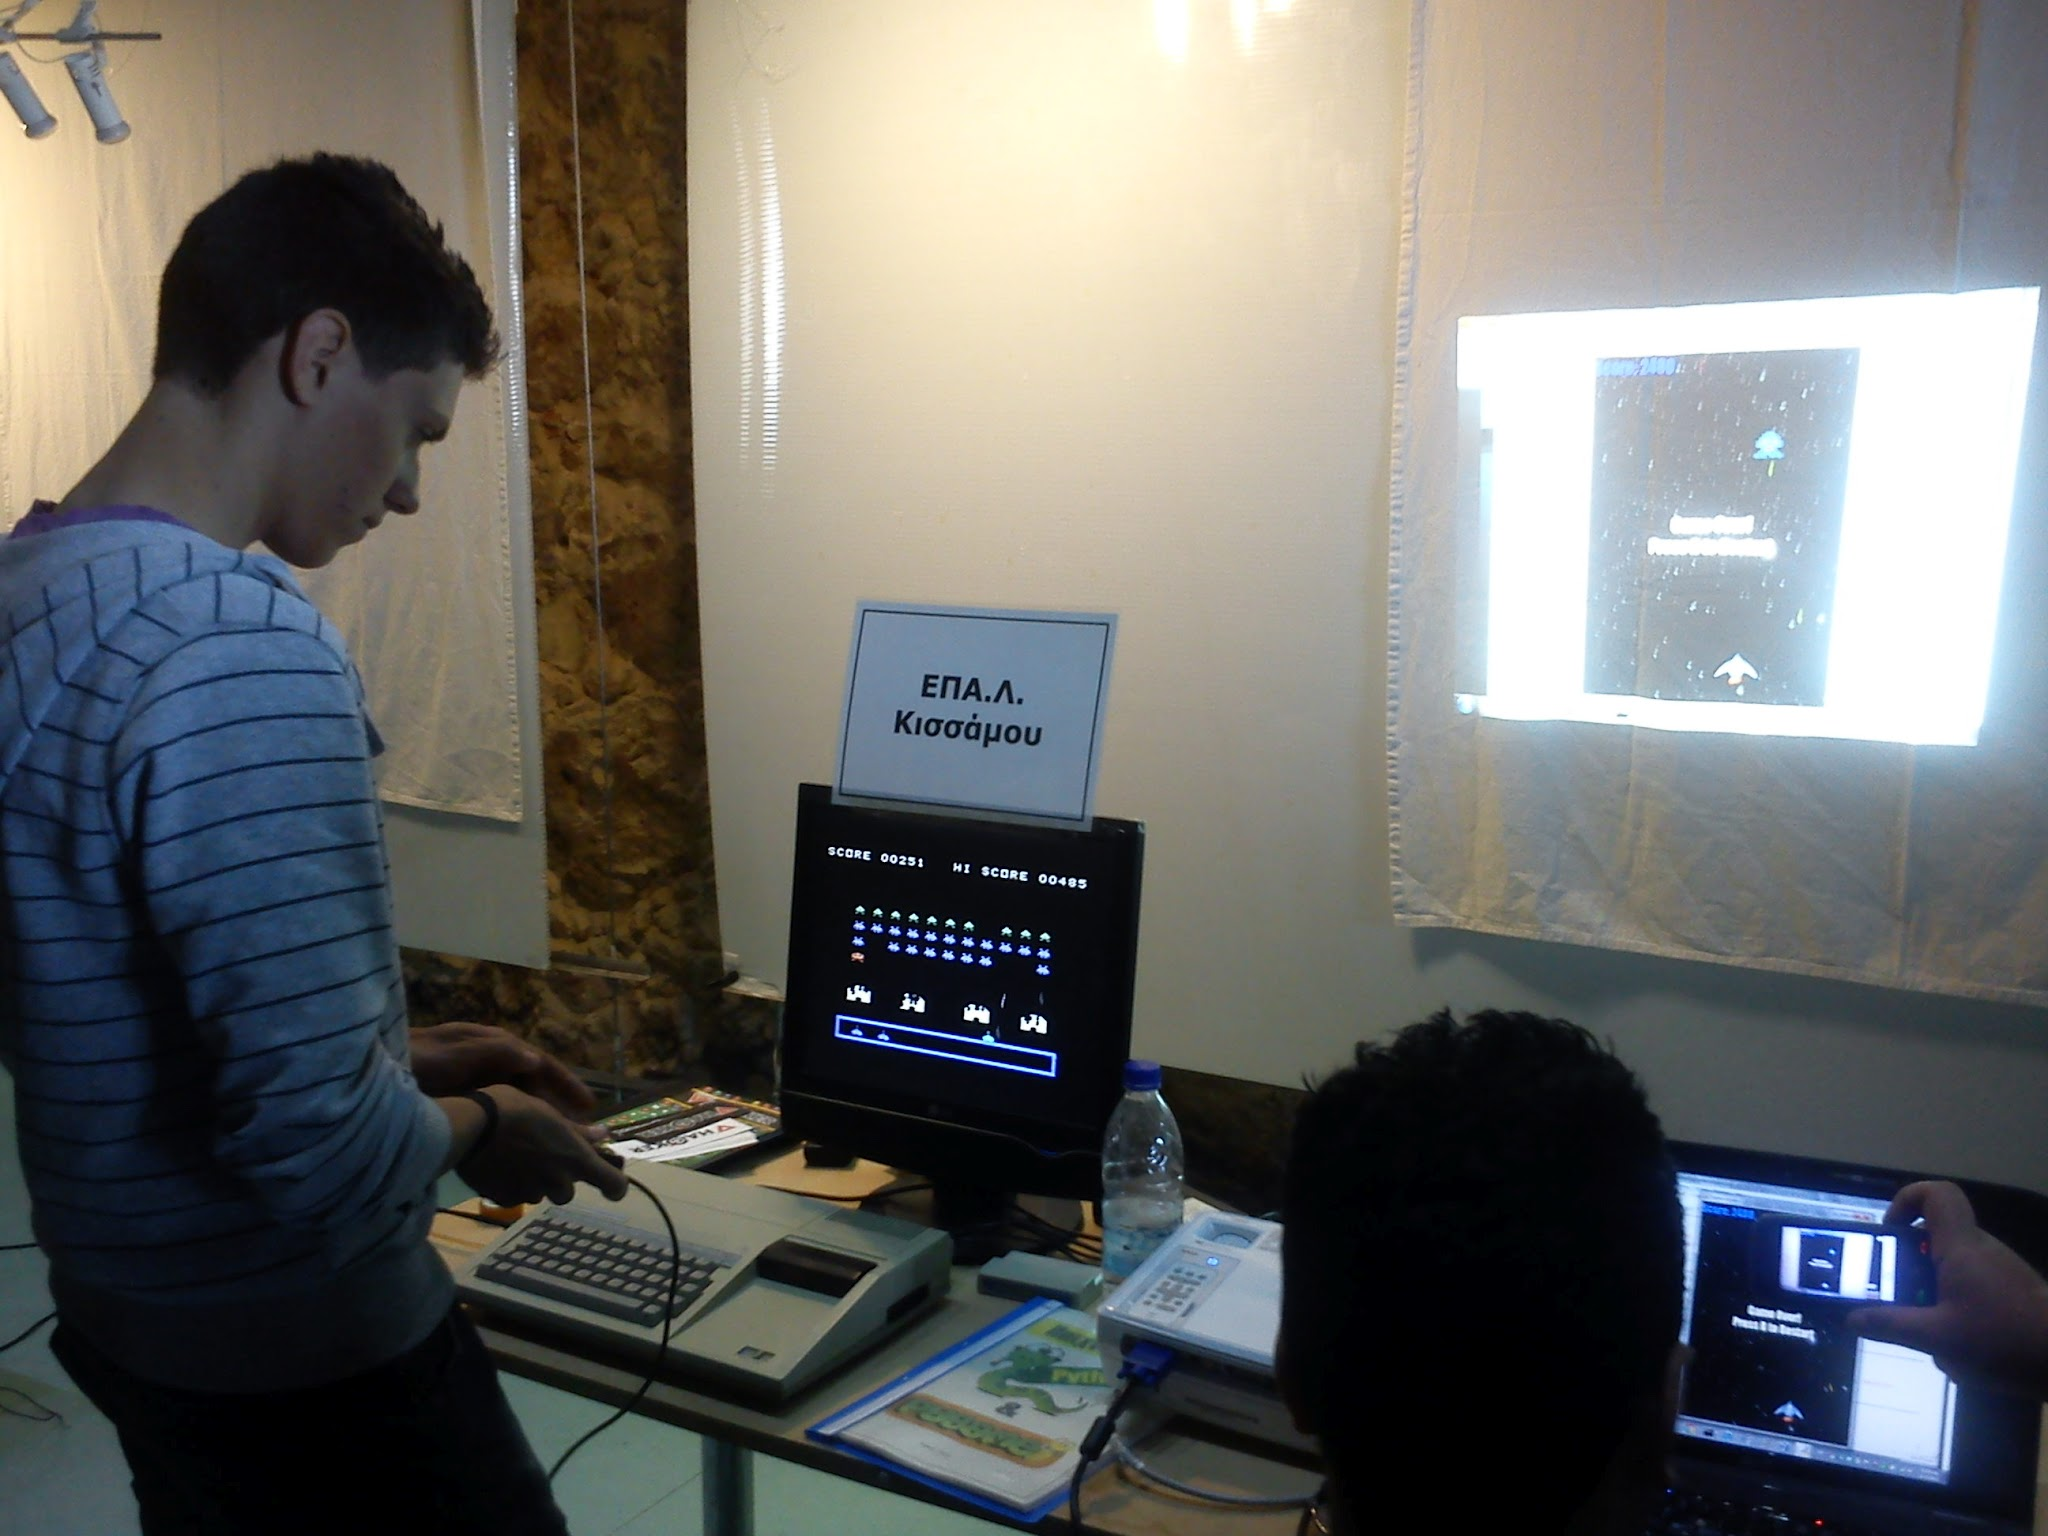
\includegraphics[width=0.8\textwidth]{images/chapter7/periptero}
\caption[Περίπτερο στην Έκθεση]{Το περίπτερο μας στην έκθεση. Ο original TI-99/4A με το cartridge TI Invaders αλλά και με δικά μου παιχνίδια σε BASIC και Extended BASIC διασκέδασε πολύ κόσμο. Τελικά το κλασικό δεν πεθαίνει ποτέ (και ειδικά το συγκεκριμένο μηχάνημα είναι φτιαγμένο να αντέξει για πάντα όπως φαίνεται). Δεξιά φαίνεται στον video-προβολέα το Pygame Invaders το οποίο φυσικά ήταν το hit της έκθεσης!}
\label{7-2}
\end{figure}

\begin{minted}[bgcolor=bg, linenos, frame=lines, framesep=10pt]{python}
# Background music
import pygame
from pygame.locals import *
pygame.init()
clock = pygame.time.Clock()
pygame.mixer.music.load("spaceinvaders.ogg")
pygame.mixer.music.play()
while pygame.mixer.music.get_busy():
  clock.tick()
\end{minted}

Παρόμοια και για τη μουσική, αλλά παρατηρήστε ότι η {\tt pygame.mixer.music.load} δεν δημιουργεί κανένα αντικείμενο καθώς το κανάλι για streaming μουσικής είναι μόνο ένα.

Κάτι πολύ ενδιαφέρον όμως είναι ότι μπορούμε να γράψουμε:

\begin{minted}[bgcolor=bg, frame=lines, framesep=10pt]{python}
pygame.mixer.music.play(6)
\end{minted}

και το τραγούδι να επαναληφθεί 6 φορές. Η ακόμα:

\begin{minted}[bgcolor=bg, frame=lines, framesep=10pt]{python}
pygame.mixer.music.play(-1)
\end{minted}

οπότε θα επαναλαμβάνεται συνέχεια! Πολύ χρήσιμο για το παιχνίδι μας. Να σημειώσουμε εδώ ότι το pygame δεν τα πάει τόσο καλά με τα mp3 οπότε προτιμήστε αρχεία ogg (ή ασυμπίεστα wav για τα ηχητικά εφέ που είναι μικρά).

\begin{figure}
\centering
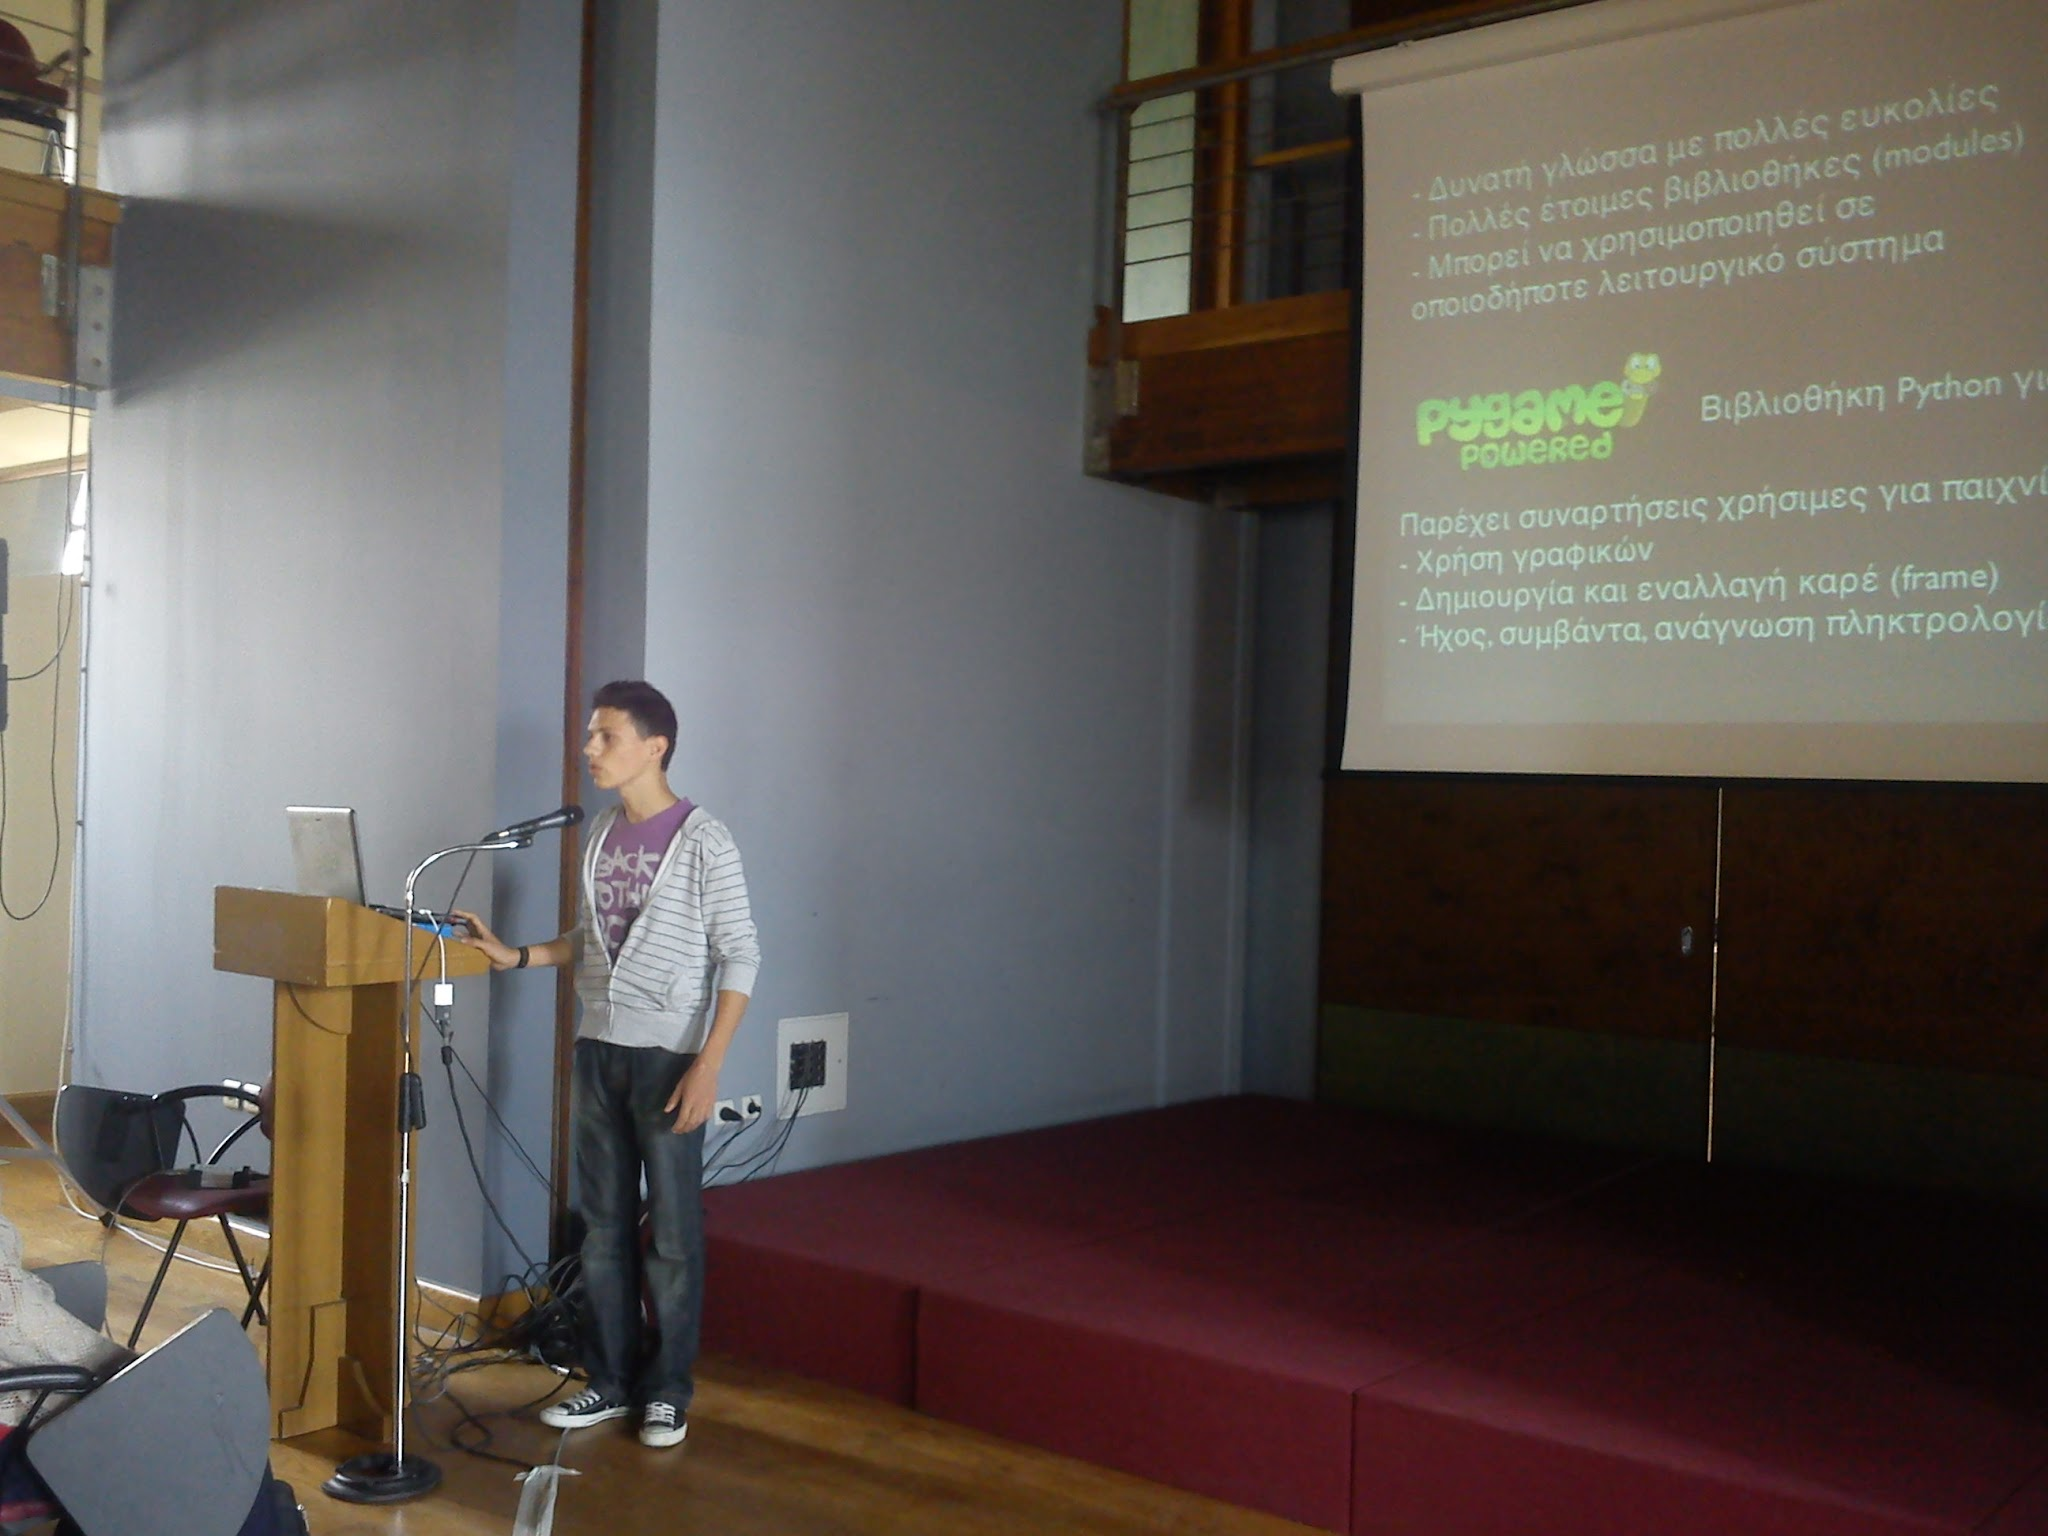
\includegraphics[width=0.8\textwidth]{images/chapter7/andreas}
\caption[Παρουσίαση Pygame]{Ο μαθητής μας Ανδρέας Κοντορίνης παρουσιάζει το pygame στην Έκθεση Μαθητικής Δημιουργίας Πληροφορικής στα Χανιά. Ο Ανδρέας υπήρξε βασικό πειραματόζ.. ε\ldots{} beta tester για τη σειρά μαθημάτων Python Game Programming.}
\label{7-1}
\end{figure}

\section{Τα Αντικείμενα του Παιχνιδιού}

Έχοντας ξεκαθαρίσει κάπως τα πράγματα με τον ήχο, ώρα να σκεφτούμε λίγο τα αντικείμενα του παιχνιδιού και τι κλάσεις θα χρειαστεί να δημιουργήσουμε. Έχουμε λοιπόν:
%
\begin{enumerate}
\item Το διαστημοπλοιάκι μας
\item Τους εξωγήινους
\item Το laser μας
\item Το laser των εξωγήινων (μακριά από μας!)
\item Το φόντο
\end{enumerate}
%
Ίσως να μπείτε στον πειρασμό να φτιάξετε μια κλάση για το καθένα από αυτά, αλλά μη βιαστείτε. Όχι ότι θα είναι λάθος αν το κάνετε, αλλά θα βρεθείτε να γράφετε τον ίδιο κώδικα δύο φορές.  Γιατί αν το σκεφτείτε καλύτερα:
%
\begin{itemize}
\item Το διαστημοπλοιάκι μας και οι εξωγήινοι ουσιαστικά είναι παρόμοια αντικείμενα και χρειάζονται παρόμοιες μεθόδους.
\item Οι δικές μας βολές laser ελάχιστα διαφέρουν από των εξωγήινων: ουσιαστικά στην κατεύθυνση της κίνησης και στον\ldots{} στόχο.
\end{itemize}
%
Τι μεθόδους χρειαζόμαστε για το δικό μας σκάφος; Αν μελετήσατε την object oriented εκδοχή του bouncing ball στο Κεφάλαιο \ref{chap:objects-intro}, θα μπορέσετε να σκεφτείτε εύκολα:
%
\begin{itemize}
\item Τη μέθοδο {\tt Show} για να απεικονίζεται σε μια επιφάνεια που θα δώσουμε ως παράμετρο.
\item Τη μέθοδο {\tt Move} για να κινείται στην οθόνη.
\item Τη μέθοδο {\tt Fire} για να ρίχνει (ok, αυτό είναι καινούριο. Δεν έχουμε δει πουθενά bouncing balls που να πυροβολούν)
\item Ένα constructor που να το δημιουργεί (να φορτώνει την εικόνα, να βρίσκει τις διαστάσεις κλπ)
\end{itemize}
%
Τις ίδιες όμως μεθόδους χρειάζεται και ο εξωγήινος! Η υλοποίηση θα διαφέρει σε ορισμένες μεθόδους -- αλλά αν φτιάξουμε πρώτα μια γενική κλάση ({\em υπερκλάση ή superclass}) για τα διαστημόπλοια μπορούμε μετά να εξειδικεύσουμε τις μεθόδους όπου χρειάζεται.

\section{Η Υπερκλάση Craft}

Σε μια πρώτη σκέψη μπορούμε να γράψουμε την παρακάτω:

\begin{minted}[bgcolor=bg, linenos, frame=lines, framesep=10pt]{python}
class Craft(object):
  def __init__ (self, imagefile, coord):
    self.shape = pygame.image.load(imagefile)
    self.ship_width = self.shape.get_width()
    self.ship_height = self.shape.get_height()
    self.rect = pygame.Rect(coord,(self.ship_width, self.ship_height))

  def Show(self, surface):
    surface.blit(self.shape,(self.rect[0],self.rect[1]))

  def Move(self,speed_x,speed_y, time):
    distance_x = speed_x * time
    distance_y = speed_y * time
    self.rect.move_ip(distance_x,distance_y)

  def Fire(self):
    pass
\end{minted}

\begin{SCfigure}
\centering
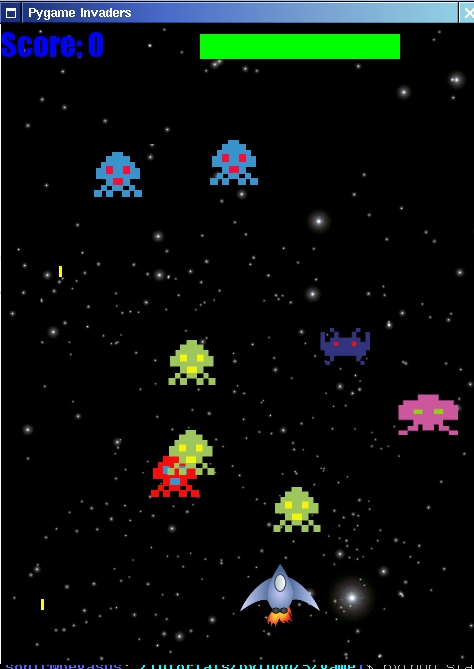
\includegraphics[width=0.5\textwidth]{images/chapter7/pygame-invaders}
\caption[Pygame Invaders!]{Το παιχνίδι μας όπως θα δείχνει σε κάποιο προχωρημένο στάδιο. Παρατηρήστε τους retro εξωγήινους που προέρχονται από το αρχικό Space Invaders και το δικό μας υπερσύγχρονο διαστημόπλοιο. Δεν είναι τυχαίο που τελικά ποτέ δεν κυρίευσαν τη γη με αυτές τις μπακατέλες που έρχονταν. Eat my laser alien!}
\label{7-3}
\end{SCfigure}

Μερικές γρήγορες παρατηρήσεις:

Αντί να χρησιμοποιούμε χωριστές μεταβλητές για να κρατάμε τις συντεταγμένες του διαστημοπλοίου, χρησιμοποιούμε το {\tt Rect} class του pygame. Αυτό δημιουργεί αντικείμενα τύπου ``παραλληλόγραμμο'' τα οποία ουσιαστικά είναι λίστες με τέσσερα στοιχεία:

\begin{verbatim}
[ Θέση_Χ, Θέση_Y, Πλάτος, Ύψος ]
\end{verbatim}

Έτσι π.χ. η εντολή:

\begin{minted}[bgcolor=bg, frame=lines, framesep=10pt]{python}
rect = pygame.Rect((240,560),(100,100))
\end{minted}

φτιάχνει ένα αντικείμενο {\tt rect} το οποίο είναι:

\begin{minted}[bgcolor=bg, frame=lines, framesep=10pt]{python}
[240, 560, 100, 100]
\end{minted}

Το καλό με την κλάση {\tt Rect} είναι ότι περιέχει μεθόδους για να κινήσουμε το αντικείμενο μας --- ουσιαστικά δηλαδή να αλλάξουμε τις συντεταγμένες Χ και Υ --- αλλά κυρίως για να δούμε αν ένα αντικείμενο {\tt rect} βρίσκεται μέσα σε ένα άλλο (hint: αν έχουμε χτυπηθεί από το laser)

Μπορείτε να δείτε και να καταλάβετε εύκολα την κίνηση στην μέθοδο {\tt Move}:

\begin{minted}[bgcolor=bg, frame=lines, framesep=10pt]{python}
    self.rect.move_ip(distance_x,distance_y)
\end{minted}

ουσιαστικά το παραπάνω αντικαθιστά τις εντολές:

\begin{minted}[bgcolor=bg, frame=lines, framesep=10pt]{python}
    x = x + distance_x
    y = y + distance_y
\end{minted}

που έχουμε δει σε προγράμματα όπως το bouncing ball. Αν πάλι κάπου χρειαζόμαστε μόνο τις τιμές των θέσεων X και Y μπορούμε να τις πάρουμε από το {\tt rect[0]} και {\tt rect[1]} αντίστοιχα, όπως φαίνεται και στη μέθοδο {\tt Show}.

Η μέθοδος {\tt Fire} περιέχει μόνο μια εντολή:

\begin{minted}[bgcolor=bg, frame=lines, framesep=10pt]{python}
    pass
\end{minted}

Την {\tt pass} τη χρησιμοποιούμε στην python όταν κάπου χρειάζεται μια εντολή αλλά εμείς δεν έχουμε κάτι να γράψουμε. Προφανώς τη μέθοδο {\tt Fire} δεν την έχουμε σκεφτεί ακόμα, βάζουμε λοιπόν {\tt pass} προκειμένου να την ολοκληρώσουμε αργότερα.

Από την υπερκλάση {\tt Craft} θα δημιουργήσουμε τις κλάσεις για το δικό μας διαστημόπλοιο αλλά και για τους εξωγήινους. Θα ξεκινήσουμε με μια απλή εκδοχή:

\begin{minted}[bgcolor=bg, frame=lines, framesep=10pt]{python}
class SpaceCraft(Craft):
  pass
\end{minted}

Καθώς καταλαβαίνετε, σίγουρα θα προσθέσουμε πράγματα σε αυτή την κλάση αλλά για την ώρα ας δούμε πως λειτουργεί στην πλέον βασική της μορφή -- χωρίς καμιά διαφορά από την υπερκλάση.

\section{Μια Κλάση για το Background (Φόντο)}

Έχουμε βρει μια ωραία φώτο με αληθινά αστέρια την οποία θα χρησιμοποιήσουμε ως φόντο. Μελλοντικά θέλουμε να την κάνουμε να σκρολλάρει κατακόρυφα (και ελπίζουμε ότι μέσα στον πυρετό της μάχης ο παίκτης δεν θα παρατηρήσει ότι είναι η ίδια εικόνα που επαναλαμβάνεται!). Για την ώρα θα αρκεστούμε σε μια στατική απεικόνιση:

\begin{minted}[bgcolor=bg, linenos, frame=lines, framesep=10pt]{python}
class SpaceBackground:
  def __init__(self, coord, imagefile):
    self.shape = pygame.image.load(imagefile)
    self.coord = coord

  def Show(self, surface):
    surface.blit(self.shape,self.coord)

  def Scroll(self, speed_y, time):
    pass
\end{minted}

Είναι εξαιρετικά απλή φυσικά: Ο constructor δέχεται μόνο το όνομα αρχείου
της εικόνας. Έχουμε φροντίσει το μέγεθος να είναι ίδιο με το παράθυρο, οπότε
η απεικόνιση θα γίνει στη θέση (0,0). Η μέθοδος {\tt Show} κλασικά εμφανίζει το
φόντο πάνω στην επιθυμητή επιφάνεια ενώ η μέθοδος Scroll θα κάνει το φόντο
να κυλάει κατακόρυφα με την επιθυμητή ταχύτητα {\tt speed\_y}. Όταν φυσικά μας έρθει η θεία επιφώτιση να την γράψουμε, γιατί για την ώρα το φόντο θα είναι στατικό.

\section{Το Κύριο Πρόγραμμα}

Για την ώρα είναι αρκετά εύκολο:

\begin{minted}[bgcolor=bg, frame=lines, framesep=10pt]{python}
  pygame.init()
  screenwidth,screenheight = (480,640)
\end{minted}

Το μέγεθος του παραθύρου μας

\begin{minted}[bgcolor=bg, frame=lines, framesep=10pt]{python}
  spaceship_pos = (240, 540)
\end{minted}

Η αρχική θέση του διαστημοπλοίου μας

\begin{minted}[bgcolor=bg, frame=lines, framesep=10pt]{python}
  screen = pygame.display.set_mode((screenwidth,screenheight), DOUBLEBUF, 32)
  pygame.display.set_caption("Pygame Invaders")
  pygame.key.set_repeat(1,1)
\end{minted}

Με το {\tt pygame.key.set\_repeat(1,1)} ρυθμίζουμε την ταχύτητα αντίδρασης και επανάληψης του πληκτρολογίου σε όσο πιο γρήγορα γίνεται!

\begin{minted}[bgcolor=bg, frame=lines, framesep=10pt]{python}
  StarField = SpaceBackground("stars.jpg")
\end{minted}

Δημιουργούμε το αντικείμενο του φόντου.

\begin{minted}[bgcolor=bg, frame=lines, framesep=10pt]{python}
  SpaceShip = SpaceCraft("spaceship2.png",spaceship_pos)
\end{minted}

Δημιουργούμε το σκάφος μας στην αρχική του θέση

\begin{minted}[bgcolor=bg, frame=lines, framesep=10pt]{python}
  clock = pygame.time.Clock()
  framerate = 60
\end{minted}

Δημιουργούμε το γνωστό αντικείμενο ``ρολόι'' και εισερχόμαστε στον κύριο βρόχο:

\begin{minted}[bgcolor=bg, linenos, frame=lines, framesep=10pt]{python}
  while True:
    time = clock.tick(framerate)/1000.0
    shipspeed_x = 0
    shipspeed_y = 0
\end{minted}

Μηδενίζουμε την ταχύτητα του σκάφους. Για να κινηθεί πρέπει να πατήσουμε κάποιο πλήκτρο, διαφορετικά θα πρέπει να μένει ακίνητο στην τελευταία γνωστή του θέση!

\begin{minted}[bgcolor=bg, linenos, frame=lines, framesep=10pt]{python}
    for event in pygame.event.get():
      if event.type == QUIT:
        pygame.quit()
        exit()
      if event.type == KEYDOWN:
        # This returns a list of True/False where the index is the
        # code of the key pressed. Fortunately pygame.locals provides
        # symbolics for these codes
        key = pygame.key.get_pressed()
\end{minted}

\begin{minted}[bgcolor=bg, linenos, firstnumber=10, frame=lines, framesep=10pt]{python}
        if key[K_q]:
          pygame.quit()
          exit()
        if key[K_LEFT]:
          shipspeed_x = -300
        if key[K_RIGHT]:
          shipspeed_x = 300
\end{minted}

Για την διαχείριση των events, θα χρησιμοποιήσουμε την
{\tt pygame.key.get\_pressed()}. Αυτή επιστρέφει μια λίστα με τιμές {\tt True / False}
όπου ο δείκτης είναι ο κωδικός αριθμός του αντίστοιχου πλήκτρου. Έτσι
μπορούμε να διαβάσουμε περισσότερα από ένα πλήκτρα κάθε στιγμή (δηλ. να
μετακινούμε το διαστημόπλοιο και να ρίχνουμε βολές ταυτόχρονα). Μη ξεχνάτε
ότι το {\tt pygame.locals} δίνει συμβολικά ονόματα σε κάθε κωδικό πλήκτρου, έτσι
το πλήκτρο 113 είναι το {\tt K\_q} -- το πλήκτρο Q που θα μπορεί να πιέσει ο χρήστης για να τερματίσει το παιχνίδι. Για να ελέγξουμε λοιπόν αν πιέζεται τη δεδομένη στιγμή:

\begin{minted}[bgcolor=bg, frame=lines, framesep=10pt]{python}
        key = pygame.key.get_pressed()
        if key[K_q]:
          .... (ο παίκτης βαρέθηκε το παιχνίδι)
\end{minted}

Ευτυχώς για μας, το pygame διαβάζει με τον ίδιο τρόπο και τα βελάκια
({\tt Κ\_LEFT, K\_RIGHT}) και όποιο άλλο πλήκτρο θέλετε. Προφανώς έχουμε επιλέξει τα βελάκια για την κίνηση του σκάφους μας.

Αν πιεστεί το αριστερό βελάκι αλλάζουμε την ταχύτητα σε -300 και για το δεξιό σε 300. Αυτό ισχύει φυσικά μόνο για ένα κύκλο μέσα στο {\tt while}, γιατί όπως είδατε στην αρχή του βρόχου η ταχύτητα μηδενίζεται. Έχουμε όμως ορίσει το repeat του πληκτρολογίου σε μεγάλη ταχύτητα -- έτσι το διαστημοπλοιάκι φαίνεται να κινείται αρκετά ομαλά.

\begin{minted}[bgcolor=bg, linenos,  frame=lines, framesep=10pt]{python}
    SpaceShip.Move(shipspeed_x, shipspeed_y, time)
    StarField.Show(screen)
    SpaceShip.Show(screen)
    pygame.display.update()
\end{minted}

Κινούμε το διαστημόπλοιο, καλούμε τις αντίστοιχες μεθόδους {\tt Show} των αντικειμένων μας και φυσικά το γνωστό {\tt pygame.display.update()} για να μεταφερθούν όλα στην οθόνη μας. Απλούστατο.

Απλούστατο, αλλά δεν είναι παιχνίδι ακόμα! Που είναι οι εξωγήινοι; Που είναι
τα Laser; Που είναι ο ήχος και η μουσική; Για αυτό το τελευταίο θα κάνουμε
κάτι αμέσως. Για τα άλλα βέβαια θα χρειαστεί να διαβάσετε τις επόμενες
ενότητες.

\section{Μουσική}

Ας γράψουμε μια απλή συνάρτηση για τη μουσική του παιχνιδιού:

\begin{minted}[bgcolor=bg, frame=lines, framesep=10pt]{python}
def PlayMusic(soundfile):
  pygame.mixer.music.load(soundfile)
  pygame.mixer.music.play(-1)
\end{minted}

και αρκεί να την καλέσουμε οπουδήποτε λίγο πριν το {\tt while}:

\begin{minted}[bgcolor=bg, frame=lines, framesep=10pt]{python}
  PlayMusic("spaceinvaders.ogg")
\end{minted}

\begin{figure}
\centering
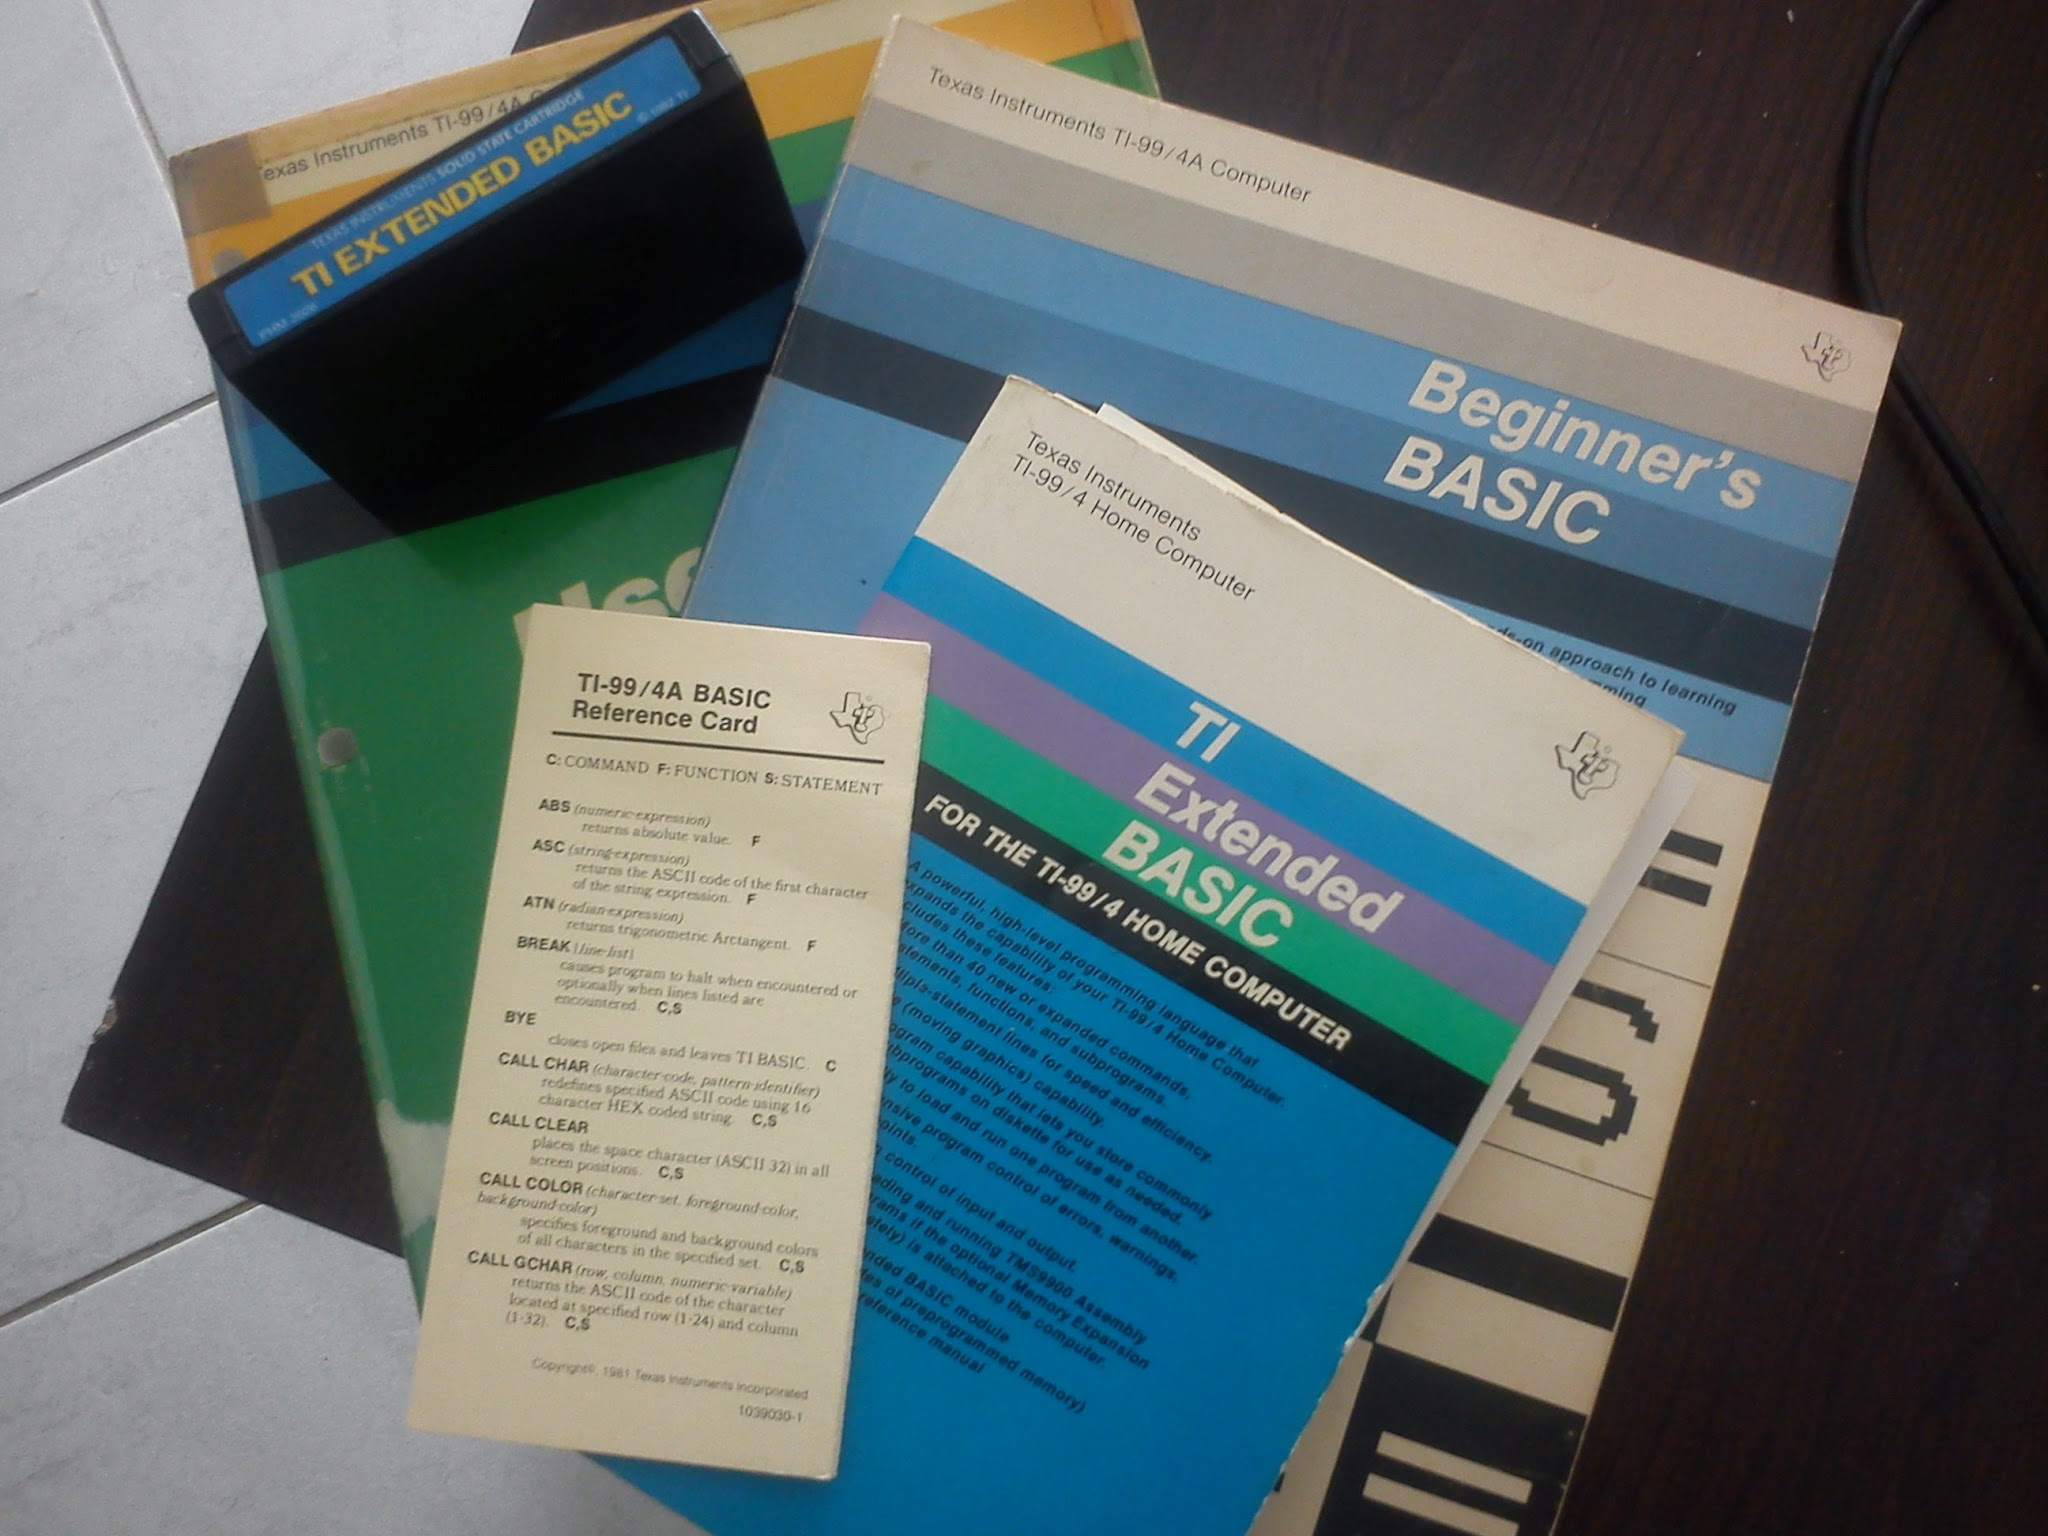
\includegraphics[width=0.8\textwidth]{images/chapter7/biblia}
\caption[Game Programming in the 80s]{Game programming στα 80s. Δεν υπήρχε
το web άρα ξεχάστε το \url{http://pygame.org}. Ότι πληροφορίες μπορούσε κανείς να βρει για τη γλώσσα περιέχονταν στα εγχειρίδια του υπολογιστή του. Εδώ βλέπετε τα βασικά βιβλία του TI-99/4A καθώς και το Extended BASIC cartridge που κόστιζε μια μικρή περιουσία. Τουλάχιστον έβγαλε τα λεφτά του (δουλεύει ακόμα\ldots{})}
\label{7-4}
\end{figure}

\section{Ευτυχώς, Έχουμε\ldots{} Προβλήματα}

Δεν φτάνει που μετά βίας έχουμε γράψει 70 γραμμές κώδικα, άρχισαν ήδη τα προβλήματα:

\begin{itemize}
\item Το διαστημοπλοιάκι κινείται αριστερά -- δεξιά και φεύγει και εκτός
οθόνης. Τι πρέπει να κάνουμε για να περιορίσουμε την κίνηση;
\item Τι γραμμές χρειάζεται για να κινείται και πάνω -- κάτω εκτός από αριστερά δεξιά;
\item Πως θα εμφανίζονται και θα κινούνται οι εξωγήινοι;
\item Πως θα πετύχουμε την κύλιση του φόντου;
\end{itemize}

Κάποια από τα παραπάνω ερωτήματα θα τα απαντήσουμε στις επόμενες ενότητες.

\section{Κίνηση Προς Όλες τις Κατευθύνσεις}

Αρχίζουμε με το δεύτερο ερώτημα που θέσαμε προηγουμένως: Πως θα κάνουμε
το διαστημόπλοιο να κινείται και πάνω -- κάτω εκτός από αριστερά -- δεξιά.
Καθώς φαντάζεστε, αυτό είναι αρκετά εύκολο, αρκεί να προσθέσετε τις παρακάτω
γραμμές σε εντελώς προφανές σημείο μέσα στον κύριο βρόχο:

\begin{minted}[bgcolor=bg, linenos, frame=lines, framesep=10pt]{python}
        if key[K_UP]:
          shipspeed_y = -300
        if key[K_DOWN]:
          shipspeed_y = 300
\end{minted}

Ναι, δεν θέλει τίποτε άλλο! Γιατί φυσικά τη ρουτίνα κίνησης την έχουμε ήδη,
το μόνο που χρειάζεται είναι να διαβάσουμε το πληκτρολόγιο και για το πάνω
και κάτω βελάκι.

Εδώ όμως μπαίνει το πρόβλημα του πρώτου ερωτήματος: Πως θα περιορίσουμε
την κίνηση του διαστημοπλοίου, το οποίο --- εκτός ότι ήδη έχει την κακή συνήθεια να ξεφεύγει αριστερά/δεξιά --- ξεφεύγει πλέον και πάνω κάτω!

Όπως φαντάζεστε οι συντεταγμένες που έχουμε για τη θέση του διαστημοπλοίου
δείχνουν αυτή τη στιγμή στην πάνω αριστερή γωνία του. Με την ευκαιρία, αυτό
δεν είναι απαραίτητο στο pygame -- μπορούμε να ορίσουμε κάποιο άλλο σημείο ως
κέντρο του αντικειμένου. Αλλά μια και το έχουμε συνηθίσει, ας συνεχίσουμε
έτσι.

Είναι μάλλον εμφανές ότι οι συντεταγμένες αυτές δεν θα πρέπει να γίνουν
μικρότερες από το (0,0) που αντιπροσωπεύει την πάνω αριστερή γωνία της οθόνης. Αλλά τι έχουμε να πούμε για τις μέγιστες συντεταγμένες;

Αν είστε λίγο βιαστικοί θα πείτε ότι οι μέγιστες είναι το (480,640) ή αν
προτιμάτε να το εκφράσουμε στα δεδομένα του προγράμματος το
{\tt (screenwidth, screenheight)}. Δεν έχετε πολύ άδικο, αλλά όπως είπα στην αρχή: είστε λίγο βιαστικοί.

Βλέπετε, το σημείο (480,640) αντιπροσωπεύει το κάτω δεξιά άκρο του
παραθύρου, ενώ το σημείο αναφοράς για το διαστημόπλοιο είναι πάνω αριστερά.
Βέβαια και στο bouncing ball έχουμε κάνει κάτι αντίστοιχο: αφαιρούμε το πλάτος
 και το ύψος του αντικειμένου και προσαρμόζουμε κατάλληλα: στην
πραγματικότητα λοιπόν οι μέγιστες συντεταγμένες θα είναι:\\
{\tt (480 - πλάτος\_διαστημοπλοίου, 640-ύψος\_διαστημοπλοίου)}.

Τώρα το ωραίο με τα αντικείμενα είναι ότι μπορούμε να φτιάξουμε την κλάση
μας με τέτοιο τρόπο ώστε να φροντίζει αυτές τις μικρές αλλά ενοχλητικές
λεπτομέρειες εσωτερικά. Δεν υπάρχει λόγος όταν στο κύριο πρόγραμμα δημιουργούμε το περίφημο μας {\tt SpaceShip} object να μην του δώσουμε σαν μέγιστες συντεταγμένες το (480,640) και να το αφήσουμε να καταλάβει μόνο του ότι πρέπει να αναλάβει να κάνει αυτές τις πράξεις ανάλογα με το μέγεθος του. Το μόνο του βέβαια
είναι τρόπος του λέγειν, καθώς φυσικά πάλι εμείς θα γράψουμε τον κώδικα.

Πως όμως θα περάσουμε αυτούς τους περιορισμούς; Μια ιδέα είναι να τις δίνουμε ως παραμέτρους κατά τη δημιουργία του αντικειμένου. Τη δεδομένη στιγμή
το αντικείμενο μας δημιουργείται με την παρακάτω εντολή:

\begin{minted}[bgcolor=bg, frame=lines, framesep=10pt]{python}
  SpaceShip = SpaceCraft("spaceship2.png",spaceship_pos)
\end{minted}

και μάλλον τώρα θέλουμε κάτι τέτοιο:

\begin{minted}[bgcolor=bg, frame=lines, framesep=10pt]{python}
  spaceship_low = (0,0)
  spaceship_high = (screenwidth, screenheight)
  SpaceShip = SpaceCraft("spaceship2.png",spaceship_pos, spaceship_low, spaceship_high)
\end{minted}

Βλέπετε ότι περνάμε τις συντεταγμένες ως δύο tuples (δεν είναι κάτι που θα
αλλάξουμε), απευθείας στον constructor του {\tt SpaceCraft} class. Για μισό
λεπτό όμως, το {\tt SpaceCraft} class δεν έχει constructor: για την ακρίβεια δεν έχει
τίποτα εκτός από ένα απλό {\tt pass}. Έτσι απλά εκτελείται ο constructor του {\tt Craft}
ο οποίος δεν γνωρίζει τίποτα για συντεταγμένες low και high! Μάλλον ήρθε η
ώρα να γράψουμε κάτι στην κλάση {\tt SpaceCraft}, δεν νομίζετε; Σβήστε λοιπόν το
{\tt pass} και πάμε να φτιάξουμε constructor:

\begin{minted}[bgcolor=bg, linenos, frame=lines, framesep=10pt]{python}
class SpaceCraft(Craft):
  def __init__ (self, imagefile, coord, min_coord, max_coord):
    super(SpaceCraft,self).__init__(imagefile,coord)
    self.min_coord = min_coord
    self.max_coord = (max_coord[0]-self.ship_width, max_coord[1]-self.ship_height)
\end{minted}

Καθώς βλέπετε, το πρώτο πράγμα που θα κάνει ο constructor του {\tt
SpaceCraft} είναι να καλέσει τον αντίστοιχο της γονικής κλάσης {\tt Craft} με την εντολή:

\begin{minted}[bgcolor=bg, frame=lines, framesep=10pt]{python}
    super(SpaceCraft,self).__init__(imagefile,coord)
\end{minted}

Θυμηθείτε ότι για να δουλέψει αυτό, θα πρέπει η γονική κλάση να προέρχεται
από την κλάση {\tt object}, όπως και πράγματι συμβαίνει:

\begin{minted}[bgcolor=bg, frame=lines, framesep=10pt]{python}
class Craft(object):
\end{minted}

Τα δεδομένα που δίνουμε για τις ελάχιστες και μέγιστες συντεταγμένες
αποθηκεύονται στις μεταβλητές (tuple) {\tt self.min\_coord} και
{\tt self.max\_coord}. Για τις ελάχιστες δεν απαιτείται καμιά διόρθωση, ενώ για τις μέγιστες φυσικά γίνεται το γνωστό κόλπο με το πλάτος και ύψος του αντικειμένου. Αυτά τα έχει ήδη υπολογίσει
ο constructor του {\tt Craft} για εμάς!

Το γεγονός βέβαια ότι δώσαμε περιορισμούς δεν σημαίνει ότι το διαστημόπλοιο
 μας τις τηρεί κιόλας. Γιατί θα πρέπει να κάνουμε κάτι και στην {\tt Move} η οποία
δεν ελέγχει αν οι τρέχοντες συντεταγμένες είναι εκτός ορίων. Και πως να το
κάνει άλλωστε, αφού είναι μόνο η βασική {\tt Move} που έχουμε γράψει για το {\tt
Craft}
 superclass. Ώρα λοιπόν να φτιάξουμε μια {\tt Move} και στο {\tt SpaceCraft}:

\begin{minted}[bgcolor=bg, linenos, frame=lines, framesep=10pt]{python}
  def Move(self, speed_x, speed_y, time):
    super(SpaceCraft,self).Move(speed_x, speed_y, time)
    for i in (0,1):
      if self.rect[i] < self.min_coord[i]:
        self.rect[i] = self.min_coord[i]
      if self.rect[i] > self.max_coord[i]:
        self.rect[i] = self.max_coord[i]
\end{minted}

Τι κάνουμε εδώ; Μα κάτι πολύ απλό στα αλήθεια. Αφήνουμε την {\tt Move} της
γονικής κλάσης να κάνει τη δουλειά της και έπειτα βλέπουμε τις συντεταγμένες
που προέκυψαν: Αν είναι μικρότερες ή μεγαλύτερες από το όριο, απλά τις
φέρνουμε ακριβώς στο όριο. Πολύ απλά, αν πάτε σε μια άκρη της οθόνης και
συνεχίζετε να πιέζετε το βελάκι, το διαστημόπλοιο θα μείνει εκεί, ακίνητο.
No motion. No sir. Nada, nope.

Έχοντας ολοκληρώσει τη βασική κίνηση του σκάφους μας, μας μένουν ακόμα:
%
\begin{itemize}
\item Οι βολές μας
\item Κάποιο εφέ που να δείχνει ότι έχουμε χτυπηθεί (ηχητικό και οπτικό)
\item Η ασπίδα και η μέτρηση του score
\end{itemize}
%
Ακόμα δεν έχουμε αγγίξει τους εξωγήινους! Καθώς φαντάζεστε έχουμε αρκετή
δουλειά ακόμα!

\section{Μια Συνάρτηση για τον Ήχο}

Αυτό είναι επίσης πολύ εύκολο:

\begin{minted}[bgcolor=bg, frame=lines, framesep=10pt]{python}
def PrepareSound(filename):
  sound = pygame.mixer.Sound(filename)
  return sound
\end{minted}

Το οποίο θα μπορείτε να το καλέσετε κάπως έτσι:

\begin{minted}[bgcolor=bg, frame=lines, framesep=10pt]{python}
explosion = PrepareSound("explosion.wav")
\end{minted}

Και φυσικά ο ήχος θα είναι έπειτα διαθέσιμος για χρήση σε οποιοδήποτε σημείο του προγράμματος τον χρειάζεστε:

\begin{minted}[bgcolor=bg, frame=lines, framesep=10pt]{python}
explosion.play()
\end{minted}
